\pagenumbering{gobble}
	\underline{\textbf{Architectural design} }
	\begin{legal}
    	\item \textit{\textbf{Overview: high-level components and their interaction}}\\\\
The figure below represents an high level overview of the system. Further details
on the system components and their interaction will be further explained in the next sections.\\
		\begin{figure}[H]
		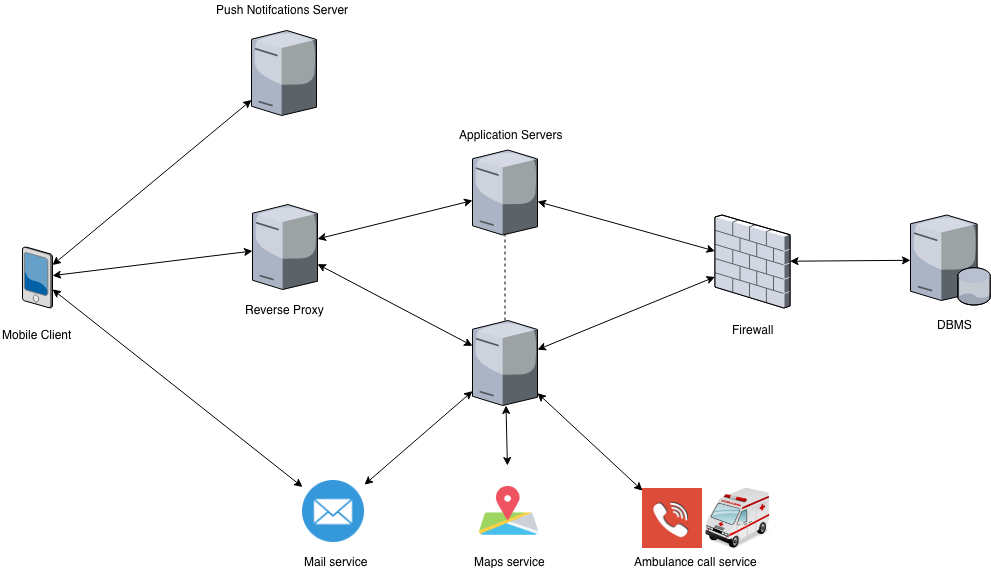
\includegraphics[width=\linewidth]{../images/design/OverviewDiagram.png}
		\end{figure}
		
		\item \textit{\textbf{Component view}}\\\\
		\begin{figure}[H]
		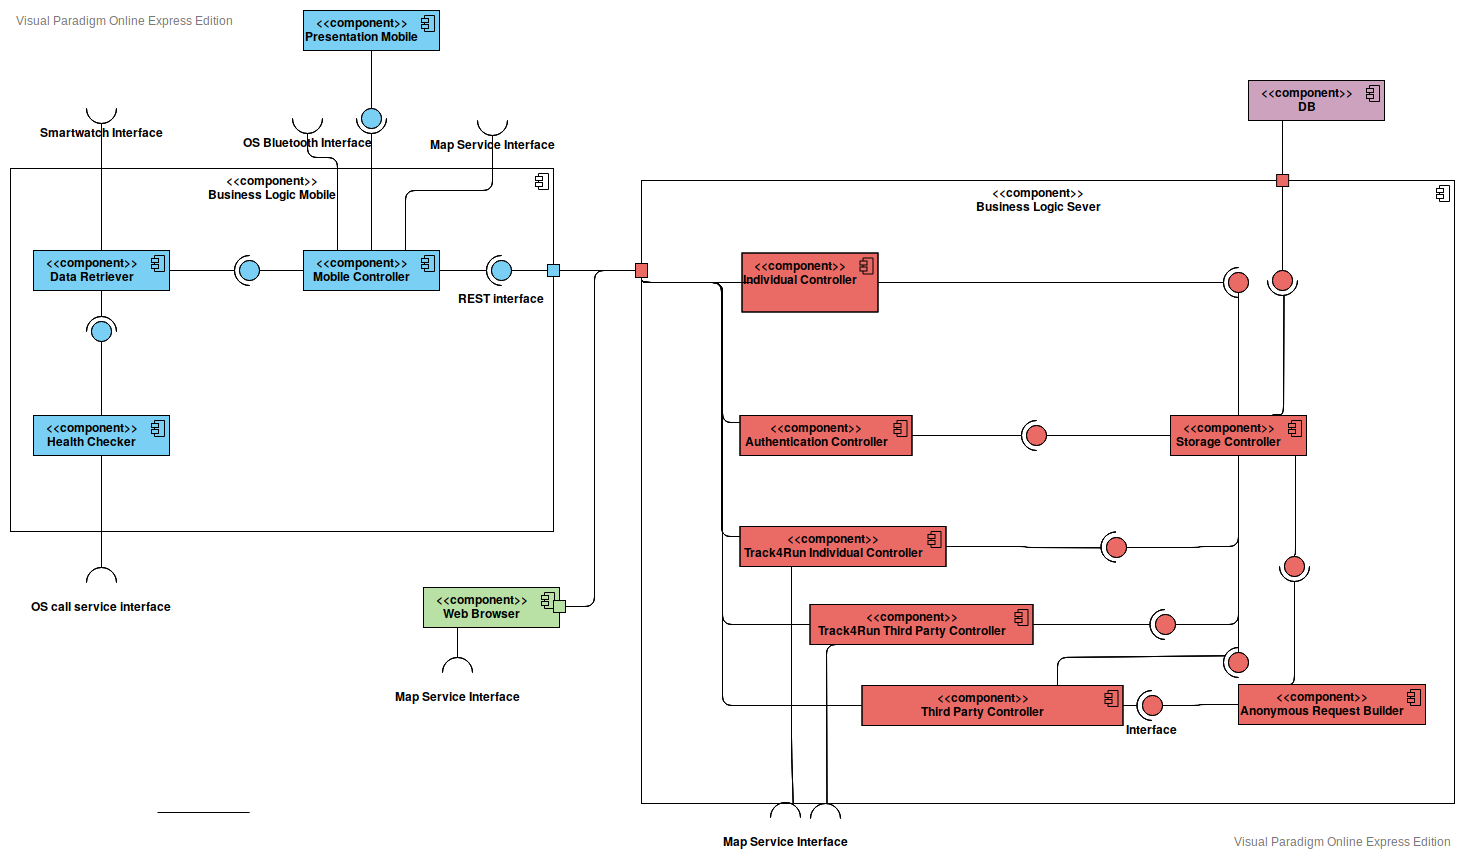
\includegraphics[width=\linewidth]{../images/design/ComponentDiagram.png}
		\end{figure}
		The UML component diagram shows the internal structure of the system highlighting the individual modules and the connections among them. It models the static implementation view of a system by breaking it down into various high levels of functionality.  Individual components are wired together by using an assembly connector to connect the required interface of one component with the provided interface of another component. For simplicity reasons, the interfaces between REST controllers (Individual, Third Party, Track4Run Individual and Track4Run Third Party Controller) and the Authentication Controller have not been drawn in the diagram. However they are present in the system in order to validate the successive user sessions after the log in. Below is the description of the components:\\
		\begin{itemize}
		\item{\textbf{Mobile Controller}\\
		This is the component that allows the individual mobile application to access to the API of the Business Logic Server. It implements the interface dedicated to the transfer of data from client to server and it translates the individual user interactions in REST API calls. If internet connection is not available or it's too slow, older health and location data are not saved locally but discarded by giving priority to new data.
				}\\
		\item{\textbf{Data Retriever}\\
		This component retrieves health data from smartwatches or similar devices, it filters them and forwards them to the Health Checker component, if the AutomatedSOS service is enabled, and to the Mobile Controller component.
				}\\
		\item{\textbf{Health Checker}\\
		This component analyzis in real time health data of the individual and checks if his or her health is fine. If it's not it interact with the operating system of the running application in order to make a SOS call.
				}\\
		\item{\textbf{Presentation}\\
		This is the component that is aimed to display the front-end content to the individual and to allow him or her to interact with the application.
				}\\
		\item{\textbf{Web Browser}\\
		The system allows the third party to interact with it through any web browser.
				}\\
		\item{\textbf{Individual Controller}\\
		The main role of this component is to manage the data coming from the specific individual by invoking the proper methods of the Storage Controller. It also provides methods to accept/refuse a request of agreement and to change personal information or preferences. Furthermore it notify to the client if there are new requests or info for him.
				}\\
		\item{\textbf{Third Party Controller}\\
		This component provides methods that allow the third party to send invidual and anonymous requests to the system. If there are new individual agreements or new data available, it sends them to the third party.
				}\\
		\item{\textbf{Authentication Controller}\\
		This component provides authentication and registration processes for both the individuals and the third parties.
				}\\
		\item{\textbf{Track4Run Individual Controller}\\
		This component provides the methods to permit an individual to join, leave, check and watch a run. It communicates with the external service that provides maps trough the Map services interface. Every time a user wants to join a run, it checks if all the constraints are satisfied. Finally, it keeps updated the individual about new info by sending him or her notifications.
				}\\
		\item{\textbf{Track4Run Third Party Controller}\\
		This component provides the methods to allow a third party to organize a run. It communicates with the external service that provides maps trough the Map services interface to allow the third party to select the track for the run.
				}\\				
		\item{\textbf{Storage Controller}
		This component provides the methods for querying and updating the Database.
				}\\
		\item{\textbf{Anonymous Request Builder}
		This component aggregates data in order to answer to third party group requests by assuring anonymity.
				}\\
		\item{\textbf{Database}
		This component represent the DBMS. It provides the interfaces to retrieve and store data. In the database there are data about users, third parties and the set of agreements among them. It also contains data about the runs.
				}\\
		\item{\textbf{External services interfaces}\\
		These interfaces are not implemented by the system but are provided by external services in order to run the application.
      	\begin{itemize}
		  	\item{\textbf{Map Service Interface}\\\
		  	It allows the third party to select the track and to show the position of runners in real time on the map.
						}\\
			\item{\textbf{OS Call Service Interface}\\
			It allows the mobile application to make a SOS phone call in case of emergency.
						}\\
			\item{\textbf{OS Bluetooth Interface}\\
			It allows the mobile application to connect the smartphone to smartwatches or similar devices.
						}\\
			\item{\textbf{Smartwatch Interface}\\
			It allows the mobile application to get data from smartwatches.
						}\\
      	\end{itemize}
				}
		\end{itemize}

		\item \textit{\textbf{Deployment view}}\\\\
		The figure below shows the deployment diagram of the whole system. Its main goal is to describe the distribution of components capturing the topology of the
system's hardware.\\
		\begin{figure}[H]
		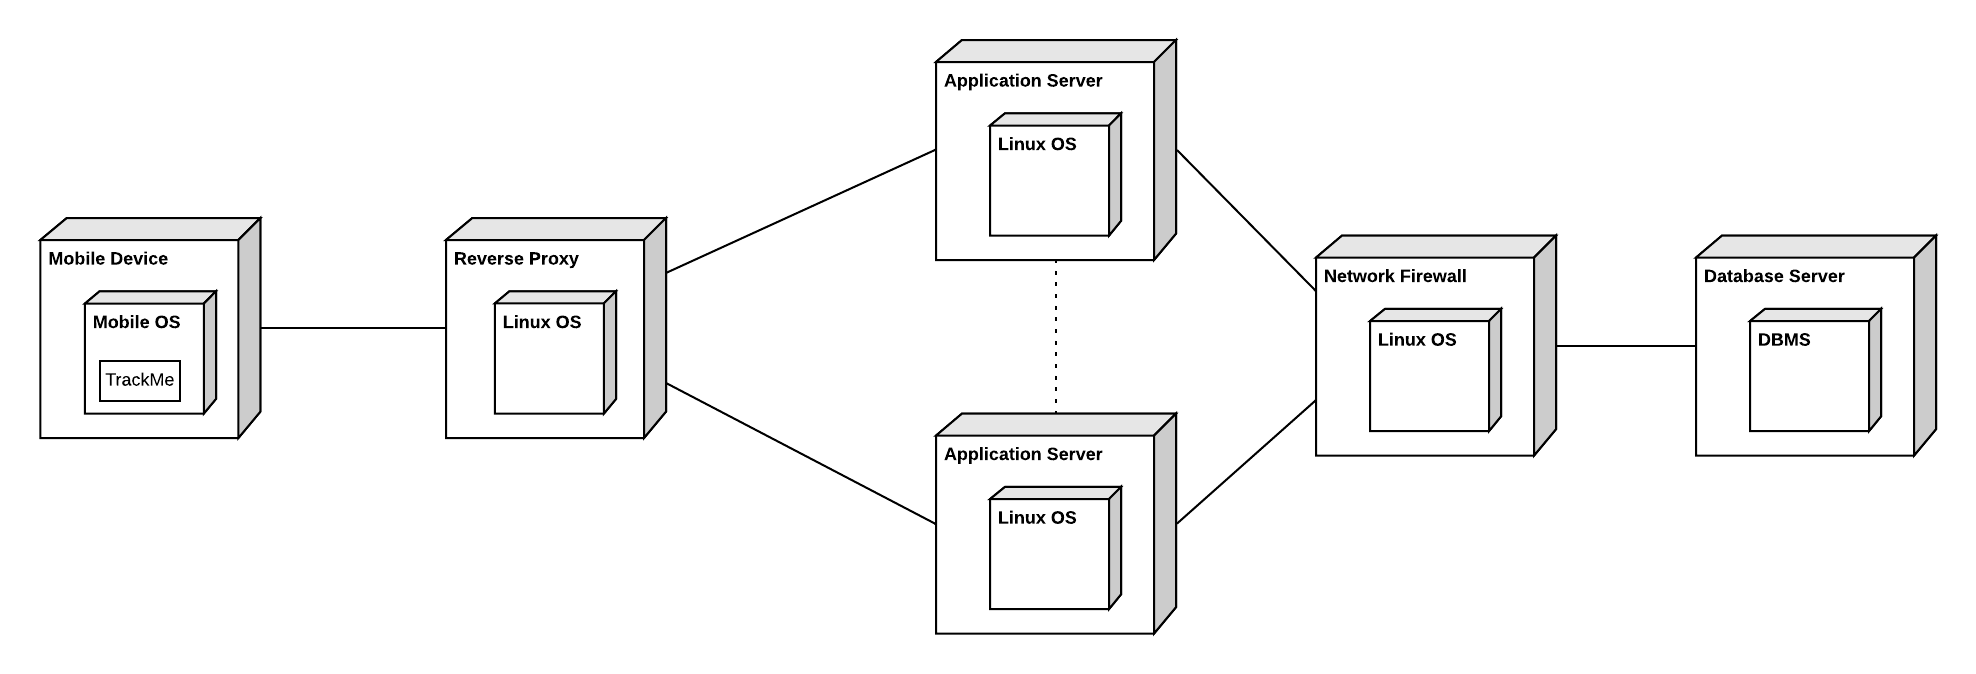
\includegraphics[width=\linewidth]{../images/design/DeploymentDiagram.png}\\
		\end{figure}
		As previously stated in the section 1, the system is structured in a multi-tier architecture. The specific role of each node is clarified here:\\\\
		\textbf{Clients}\\
The first tier is composed by the clients machines (mobile for individuals and desktop for third parties). The individuals will be able to access TrackMe functionalities through the dedicated native application while the third parties through any web browser.\\\\
		\textbf{Application Server}\\
This is the middleware level of the architecture: all the business logic of
the system is contained in this server.\\\\
		\textbf{Network Firewall}\\
The access to the Database is mediated by a network firewall in order to
avoid unauthorised access to the data and the credentials of the user.\\\\
		\textbf{Database Server}\\
This is the last layer of the architecture: all the data are stored in a Database Server accessed through a relational DBMS. \\\\

		\item \textit{\textbf{Runtime view}}\\
			\begin{legal}
				\item \textbf{Sign up Runtime View}\\
				\item \textbf{Login Runtime View}\\
				\item \textbf{Join a run Runtime View}\\
				\item \textbf{Organise a run Runtime View}\\
				\item \textbf{Individual request Runtime View}\\
				\item \textbf{Group request Runtime View}\\
			\end {legal}
		\item \textit{\textbf{Component interfaces}}\\\\
			\begin{itemize}
				\item \textbf{Authentication Controller} \\
				
				\textbf{Third Party Registration} \\
			
					\begin{tabularx}{\linewidth}{| l | l |}
						\hline
						endpoint & */auth/thirdparty/register \\
						\hline
						method & POST \\
						\hline
						url params & \\
						\hline
						data params &
						\parbox{0.7\textwidth}{
							\bigskip
							VAT: [alphanumeric]\\
							password : [alphanumeric]\\
							\bigskip
						} \\
						\hline
						success response &
						\parbox{0.7\textwidth}{
							\bigskip
							code: 200\\
							Content : \{message: "Registration successful"\}
							\bigskip
						} \\
						\hline
						error response &
						\parbox{0.7\textwidth}{
							\bigskip
							code: 422 UNPROCESSABLE ENTRY \\
							Content : \{error: "Registration Data not correct"\}
							\bigskip
						} \\
						\hline
						Notes & 
						\parbox{0.7\textwidth}{
							\bigskip Allows a third party to register to the system.
						\bigskip}  \\
						\hline
					\end{tabularx}\\
					
				\textbf{Individual Registration} \\
			
					\begin{tabularx}{\linewidth}{| l | l |}
						\hline
						endpoint & */auth/individual/register \\
						\hline
						method & POST \\
						\hline
						url params & \\
						\hline
						data params &
						\parbox{0.7\textwidth}{
							\bigskip
							username: [alphanumeric]\\
							password : [alphanumeric]\\
							name: [text]\\
							surname: [text]\\
							address: [alphanumeric]\\
							age: [integer]
							\bigskip
						} \\
						\hline
						success response &
						\parbox{0.7\textwidth}{
							\bigskip
							code: 200\\
							Content : \{message: "Registration successful"\}
							\bigskip
						} \\
						\hline
						error response &
						\parbox{0.7\textwidth}{
							\bigskip
							code: 422 UNPROCESSABLE ENTRY \\
							Content : \{error: "Registration Data not correct"\}
							\bigskip
						} \\
						\hline
						Notes & 
						\parbox{0.7\textwidth}{
							\bigskip Allows an individual to register to the system.
						\bigskip}  \\
						\hline
					\end{tabularx}\\
					
					\textbf{Individual Login}\\

						\begin{tabularx}{\linewidth}{| l | l |}
							\hline
							endpoint & */auth/individual/login \\
							\hline
							method & POST \\
							\hline
							url params & \\
							\hline
							data params &
							\parbox{0.7\textwidth}{
								\bigskip
								username: [alphanumeric]\\
								password : [alphanumeric]
								\bigskip
							} \\
							\hline
							success response &
							\parbox{0.7\textwidth}{
								\bigskip
								code: 200\\
								Content : \{accessToken: [alphanumeric]\}
								\bigskip
							} \\
							\hline
							error response &
							\parbox{0.7\textwidth}{
								\bigskip
								Code: 422 UNPROCESSABLE ENTRY \\
								Content : \{error: "Login data not correct"\}\\
								Code: 401 UNAUTHORIZED \\
								Content : \{error: "Wrong username or password"\}
								\bigskip
							} \\
							\hline
							Notes & 
							\parbox{0.7\textwidth}{
								\bigskip Allows an individual to obtain an authentication Token
							\bigskip }\\
							\hline
						\end{tabularx}
						
					\textbf{Third Party Login}\\

						\begin{tabularx}{\linewidth}{| l | l |}
							\hline
							endpoint & */auth/thirdparty/login \\
							\hline
							method & POST \\
							\hline
							url params & \\
							\hline
							data params &
							\parbox{0.7\textwidth}{
								\bigskip
								VAT: [alphanumeric]\\
								password : [alphanumeric]
								\bigskip
							} \\
							\hline
							success response &
							\parbox{0.7\textwidth}{
								\bigskip
								code: 200\\
								Content : \{accessToken: [alphanumeric]\}
								\bigskip
							} \\
							\hline
							error response &
							\parbox{0.7\textwidth}{
								\bigskip
								Code: 422 UNPROCESSABLE ENTRY \\
								Content : \{error: "Login data not correct"\}\\
								Code: 401 UNAUTHORIZED \\
								Content : \{error: "Wrong VAT or password"\}
								\bigskip
							} \\
							\hline
							Notes & 
							\parbox{0.7\textwidth}{
								\bigskip Allows a third party to obtain an authentication Token
							\bigskip }\\
							\hline
						\end{tabularx}\\
						
					\item \textbf{Third Party Controller} \\
					
					\textbf{Individual Request} \\
			
					\begin{tabularx}{\linewidth}{| l | l |}
						\hline
						endpoint & */request/individual \\
						\hline
						method & POST \\
						\hline
						url params & \\
						\hline
						data params &
						\parbox{0.7\textwidth}{
							\bigskip
							accessToken: [alphanumeric]\\
							fiscalcode: [alphanumeric]\\
							newDataSubscription: [boolean]
							\bigskip
						} \\
						\hline
						success response &
						\parbox{0.7\textwidth}{
							\bigskip
							code: 200\\
							Content : \{message: "Requested received and ready to be forwarded."\}
							\bigskip
						} \\
						\hline
						error response &
						\parbox{0.7\textwidth}{
							\bigskip
							code: 401 UNAUTHORIZED \\
							Content : \{error: "Third party not logged in"\}
							code: 404 NOT FOUND \\
							Content : \{error: "Fiscalcode not present in database."\}
							Code: 422 UNPROCESSABLE ENTRY \\
							Content : \{error: "Fiscal code not correct"\}
							\bigskip
						} \\
						\hline
						Notes & 
						\parbox{0.7\textwidth}{
							\bigskip Allows the third party to do an individual request of data.
						\bigskip}  \\
						\hline
					\end{tabularx}\\
					
					\textbf{Anonymous Request} \\
			
					\begin{tabularx}{\linewidth}{| l | l |}
						\hline
						endpoint & */request/group \\
						\hline
						method & POST \\
						\hline
						url params & \\
						\hline
						data params &
						\parbox{0.7\textwidth}{
							\bigskip
							accessToken: [alphanumeric]\\
							age: [alphanumeric]\\
							latCenter: [float]\\
							lonCenter: [float]\\
							radius: [float]\\
							newDataSubscripion: [boolean]
							\bigskip
						} \\
						\hline
						success response &
						\parbox{0.7\textwidth}{
							\bigskip
							code: 200\\
							Content : \{message: "Requested received and ready to be analyzed."\}
							code: 404 NOT FOUND \\
							Content : \{error: "Fiscalcode not present in database."\}\\
							Code: 422 UNPROCESSABLE ENTRY \\
							Content : \{error: "Fiscal code not correct"\}
							\bigskip
						} \\
						\hline
						error response &
						\parbox{0.7\textwidth}{
							\bigskip
							code: 401 UNAUTHORIZED \\
							Content : \{error: "Third party not logged in"\}\\
							Code: 422 UNPROCESSABLE ENTRY \\
							Content : \{error: "Incorrect data"\}
							\bigskip
						} \\
						\hline
						Notes & 
						\parbox{0.7\textwidth}{
							\bigskip Allows the third party to do a group request of data.
						\bigskip}  \\
						\hline
					\end{tabularx}\\
					
					\textbf{Modify Third Party Password}\\
				
					\begin{tabularx}{\linewidth}{| l | l |}
						\hline
						endpoint & */thirdParty/newPassword \\
						\hline
						method & PUT \\
						\hline
						url params & \\
						\hline
						data params & 
						\parbox{0.7\textwidth}{
							\bigskip
							accessToken: [alphanumeric] \\
							(optional) newPassword: [alphanumeric]\\
							(optional) oldPassword:
							[alphanumeric]\\
							\bigskip
						} \\
						\hline
						success response &
						\parbox{0.7\textwidth}{
							\bigskip
							Code: 200\\
							Content : \{message: "Password changed correctly"\}
							\bigskip
						} \\
						\hline
						error response &
						\parbox{0.7\textwidth}{
							\bigskip
							Code: 401 UNAUTHORIZED \\
							Content : \{error: "User not logged"\}\\
							Code: 403 FORBIDDEN \\
							Content : \{error: "Current password provided is incorrect"\}\\
							\bigskip
						} \\
						\hline
						Notes & \parbox{0.7\textwidth}{
							\bigskip
							Allows a third party to change its password.
							\bigskip
						} \\
						\hline
					\end{tabularx}\\
					
					\item \textbf{Individual Controller} \\
					
						\textbf{Answer to Request} \\
			
						\begin{tabularx}{\linewidth}{| l | l |}
							\hline
							endpoint & */answerToRequest \\
							\hline
							method & POST \\
							\hline
							url params & \\
							\hline
							data params &
							\parbox{0.7\textwidth}{
								\bigskip
								accessToken: [alphanumeric]\\
								thirdPartyRequester: [alphanumeric]\\
								answer: [boolean]
								\bigskip
							} \\
							\hline
							success response &
							\parbox{0.7\textwidth}{
								\bigskip
								code: 200\\
								Content : \{message: "Answer received correctly."\}
								\bigskip
							} \\
							\hline
							error response &
							\parbox{0.7\textwidth}{
								\bigskip
								code: 401 UNAUTHORIZED \\
								Content : \{error: "Individual not logged in"\}\\
								code: 404 NOT FOUND \\
								Content : \{error: "Request not found."\}
								\bigskip
							} \\
							\hline
							Notes & 
							\parbox{0.7\textwidth}{
								\bigskip Allows the individual to accept or refuse an individual request.
							\bigskip}  \\
							\hline
						\end{tabularx}\\
				\end{itemize}
		\item \textit{\textbf{Selected architectural styles and patterns}}\\\\
			
  	\end{legal}
